\chapter{系統實作結果}

\section{引擎介紹}

\subsection{架構}
\label{sub:架構}

\subsubsection{流程圖} % (fold)
\label{ssub:流程圖}



\subsubsection{架構圖} % (fold)
\label{ssub:架構圖}

RishEngine 是由眾多模塊組合而成,就像一個大工具包一樣,給遊戲開發者提供了許多功能:

\begin{itemize}
\item{Core}
    \SubItem{核心模塊,提供了許多基礎功能,例如:檔案系統、視窗、事件、輸出入等功能}
\item{Scene}
    \SubItem{場景模塊,提供了 ECS 和一些跟遊戲物件管理的功能}
\item{Layer}
    \SubItem{提供引擎像是圖層一樣操控遊戲畫面、UI}
\item{Renderer}
    \SubItem{渲染模塊,渲染的基礎建設}
\item{Physics}
    \SubItem{物理引擎,讓東西能動起來}
\item{Particle}
    \SubItem{粒子效果}
\item{Editor}
    \SubItem{編輯器,提供了讓遊戲開發者編輯的工具}
\end{itemize}

\begin{figure}[h]
    \begin{center}
    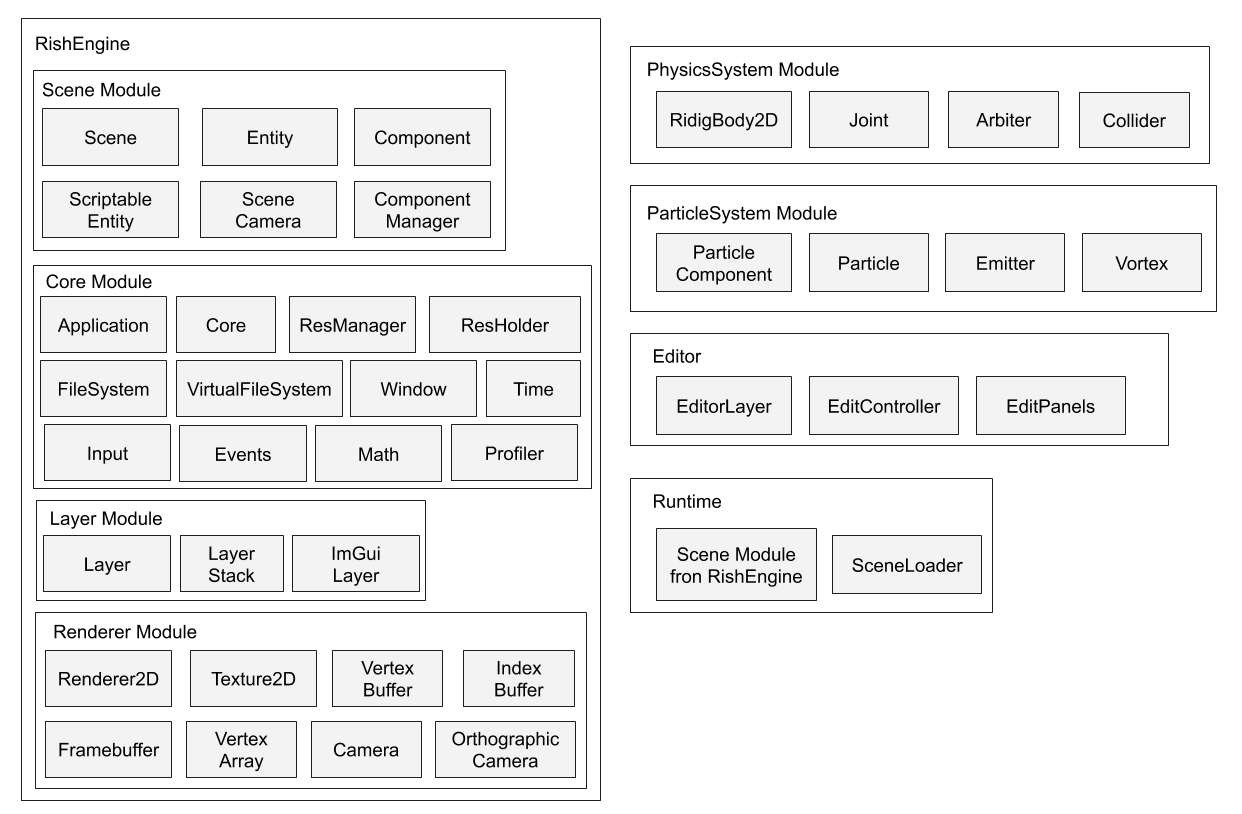
\includegraphics[width=\textwidth]{./resources/RishEngine_arch.png}
    \end{center}
\caption{RishEngine 架構}
\label{fig:RishEngineArch}
\end{figure}


%  Engine
\import{ch4/}{ecs.tex}
\import{ch4/}{batch_rendering.tex}
\import{ch4/}{particle_system.tex}
\import{ch4/}{2d_lighting.tex}
\import{ch4/}{scriptable_entity.tex}
\import{ch4/}{physics.tex}

% Editor
\import{ch4/}{editor.tex}

\newpage